Hvad kan I lave med 10 blokke?\\
I Figur~\ref{fig:blokke} ser I 10 Scratch blokke.
\begin{figure}
  \centering
  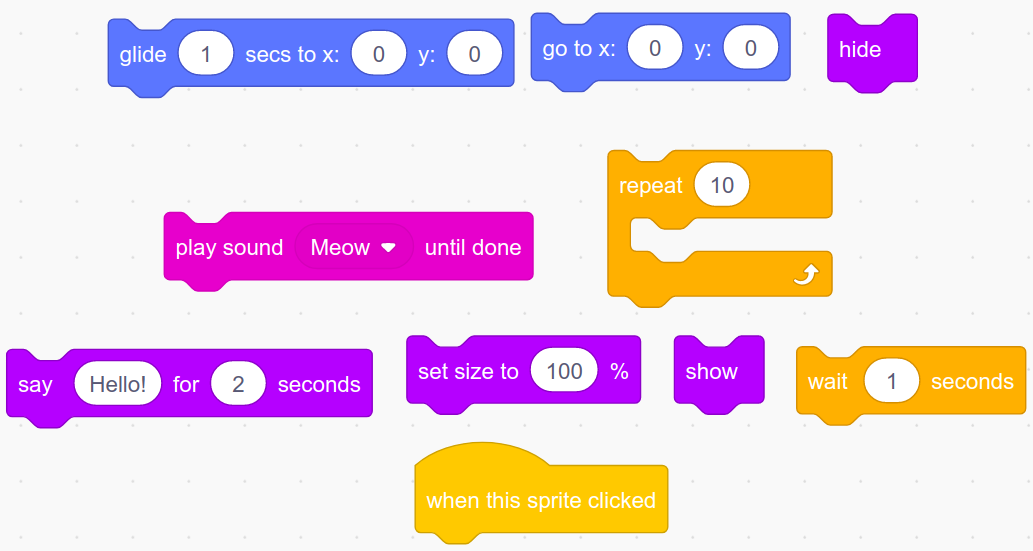
\includegraphics[width=0.9\linewidth]{figures/Scratch3.png}
  \caption{10 Scratch-blokke}
  \label{fig:blokke}
\end{figure}
Jeres opgave er at lave et sjovt program kun ved brug af disse blokke. Hver blok må bruges 0, 1 eller flere gange. Prøv at sammensætte programmet ved at tegne blokkene på papir, og skriv ned, hvad I tror programmet vil gøre. Sæt jer dernæst til computeren, og indtast jeres program. Beskriv, i hvor høj grad programmet gør, som I forventede. Vend dernæst tilbage til designfasen og forbedre evt.\ programmet. Til slut uploades programmet til gruppens studio i Scratch.
